\documentclass[final]{article}
\usepackage[paperwidth=48in,paperheight=36in,margin=0.30in]{geometry}
\usepackage{graphicx}
\usepackage[table]{xcolor}
\usepackage{booktabs}
\usepackage{array}
\usepackage{amsmath}
\usepackage{tikz}
\usepackage{hyperref}
\usepackage{lmodern}
\usepackage{microtype}
\usepackage{enumitem}
\renewcommand{\familydefault}{\sfdefault}

\pagestyle{empty}
\setlength{\parindent}{0pt}
\setlength{\parskip}{0.028in}
\setlength{\fboxsep}{0.09in}
\setlength{\fboxrule}{1.4pt}
\setlist[itemize]{leftmargin=0.24in,itemsep=0.012in,topsep=0.008in}

\definecolor{pagecream}{HTML}{F7F3E8}
\definecolor{panelwhite}{HTML}{FFFFFF}
\definecolor{templatedark}{HTML}{282622}
\definecolor{templateblue}{HTML}{0E2A55}
\definecolor{templateaccent}{HTML}{C36B4A}
\definecolor{tableblue}{HTML}{D7DEED}
\definecolor{tablebluealt}{HTML}{ECEFF7}
\definecolor{tablehead}{HTML}{38342E}
\definecolor{textblack}{HTML}{111111}

\pagecolor{templatedark}
\hypersetup{colorlinks=true,urlcolor=templateblue}

\newcounter{posterfigure}
\newcounter{postertable}

\newcommand{\bodytext}{\fontsize{16.8}{20.0}\selectfont}
\newcommand{\smalltext}{\fontsize{11.4}{13.6}\selectfont}
\newcommand{\captionfont}{\fontsize{10.3}{12.3}\selectfont}
\newcommand{\subhead}[1]{{\fontsize{18.2}{21.6}\selectfont\bfseries\color{templateblue}#1}\par}
\newcommand{\paneltitle}[1]{{\fontsize{27.5}{31.5}\selectfont\bfseries\color{textblack}#1}\par\vspace{0.030in}}
\newcommand{\contentpanel}[2]{%
  \fcolorbox{templatedark}{panelwhite}{%
    \begin{minipage}[t][#1][t]{\dimexpr\linewidth-2\fboxsep-2\fboxrule\relax}
    #2
    \end{minipage}%
  }%
}
\newcommand{\figcaption}[1]{%
  \refstepcounter{posterfigure}%
  \par\begin{center}{\captionfont\color{textblack}\textbf{Figure \theposterfigure.} #1\par}\end{center}%
}
\newcommand{\tabcaption}[1]{%
  \refstepcounter{postertable}%
  {\captionfont\color{textblack}\textbf{Table \thepostertable.} #1\par}%
  \vspace{0.018in}%
}
\newcommand{\metric}[2]{%
  \begin{minipage}[t]{0.30\linewidth}
  \centering
  {\fontsize{35}{39}\selectfont\bfseries\color{templateaccent}#1}\par
  {\smalltext\color{textblack}#2}
  \end{minipage}
}

\begin{document}
\bodytext\color{textblack}

\noindent
\colorbox{pagecream}{%
  \begin{minipage}[t][1.75in][c]{0.585\linewidth}
  {\fontsize{48}{52}\selectfont\bfseries Toward Substrate-Agnostic SERS Classification}\par
  {\fontsize{36}{41}\selectfont Using Siamese Metric Learning}
  \end{minipage}%
}
\hfill
\colorbox{templatedark}{%
  \begin{minipage}[t][1.75in][c]{0.385\linewidth}
  \raggedleft\color{white}
  {\fontsize{26.5}{30.5}\selectfont\bfseries Jesse Levine$^{1}$, Hal Bowen-Smith$^{1}$, Greg Wardle$^{1}$, and Dr. Li-Lin Tay$^{1}$}\par
  \vspace{0.08in}
  {\fontsize{18}{22}\selectfont $^{1}$Metrology Research Centre, National Research Council Canada, Ottawa, ON, Canada}\par
  \vspace{0.08in}
  {\fontsize{16}{19}\selectfont CSCCE/CIC 2026 Poster}
  \end{minipage}%
}

\vspace{0.14in}

\begin{minipage}[t]{0.49\linewidth}
\contentpanel{6.05in}{%
\paneltitle{BACKGROUND / MOTIVATION}
\subhead{Why substrate agnosticism is harder}
SERS spectra carry two coupled sources of variation: the \textbf{chemical analyte} and the \textbf{enhancing substrate}. The original model learned this combined signature well, but that does not prove chemical recognition independent of the substrate.

\subhead{The shift in target}
\textbf{Stage 1} classified measured chemical-substrate pairs such as \texttt{4np\_\_AgNP}. \textbf{Stage 2} predicts only chemical identity while holding out an entire substrate family from training.

\subhead{Central question}
Can a Siamese encoder learn a representation where spectra from the same chemical are close together even when the substrate changes?

\begin{center}
\resizebox{0.66\linewidth}{!}{%
\begin{tikzpicture}[x=1in,y=1in]
\node[draw=templatedark,fill=pagecream,rounded corners=0.07in,minimum width=3.65in,minimum height=0.78in,align=center,line width=1.1pt] (s1) at (0,0) {\textbf{Substrates}\\PICO, pSERS\\printed Ag/Au paper};
\node[draw=templatedark,fill=pagecream,rounded corners=0.07in,minimum width=3.65in,minimum height=0.78in,align=center,line width=1.1pt] (s2) at (4.25,0) {\textbf{Analyte exposure}\\Soak in diluted analyte\\for 1 h};
\node[draw=templatedark,fill=pagecream,rounded corners=0.07in,minimum width=3.65in,minimum height=0.78in,align=center,line width=1.1pt] (s3) at (8.5,0) {\textbf{Dry}\\Before measurement};
\node[draw=templatedark,fill=pagecream,rounded corners=0.07in,minimum width=3.65in,minimum height=0.78in,align=center,line width=1.1pt] (s4) at (12.75,0) {\textbf{SERS spectrum}\\Raw intensity vs.\\Raman shift};
\draw[->,line width=1.8pt,color=templateblue] (s1) -- (s2);
\draw[->,line width=1.8pt,color=templateblue] (s2) -- (s3);
\draw[->,line width=1.8pt,color=templateblue] (s3) -- (s4);
\end{tikzpicture}%
}
\end{center}
\figcaption{Sample-preparation workflow. Commercial PICO and pSERS sensors are used alongside in-house printed Ag/Au nanoparticle-paper substrates. Each analyte-substrate preparation is soaked, dried, and measured as a raw spectrum before preprocessing.}
}
\end{minipage}
\hfill
\begin{minipage}[t]{0.49\linewidth}
\contentpanel{6.05in}{%
\paneltitle{SAMPLES}
\subhead{How samples were prepared}
Two substrate types were measured: commercial PICO/pSERS sensors and in-house Ag/Au nanoparticle paper. The Ag/Au substrates were prepared by inkjet-printing colloidal nanoparticle solution onto filter paper. For each chemical-substrate condition, the substrate was soaked in a diluted analyte solution for 1 h, removed, allowed to dry, and then measured by SERS as raw intensity versus Raman shift.

\subhead{Current chemical-by-substrate matrix}
After grouping AgNP with Ag and AuNP with Au, benzenethiol and pyridine span all four substrate families. 4NP is missing on Au because it does not respond there.

\begin{center}
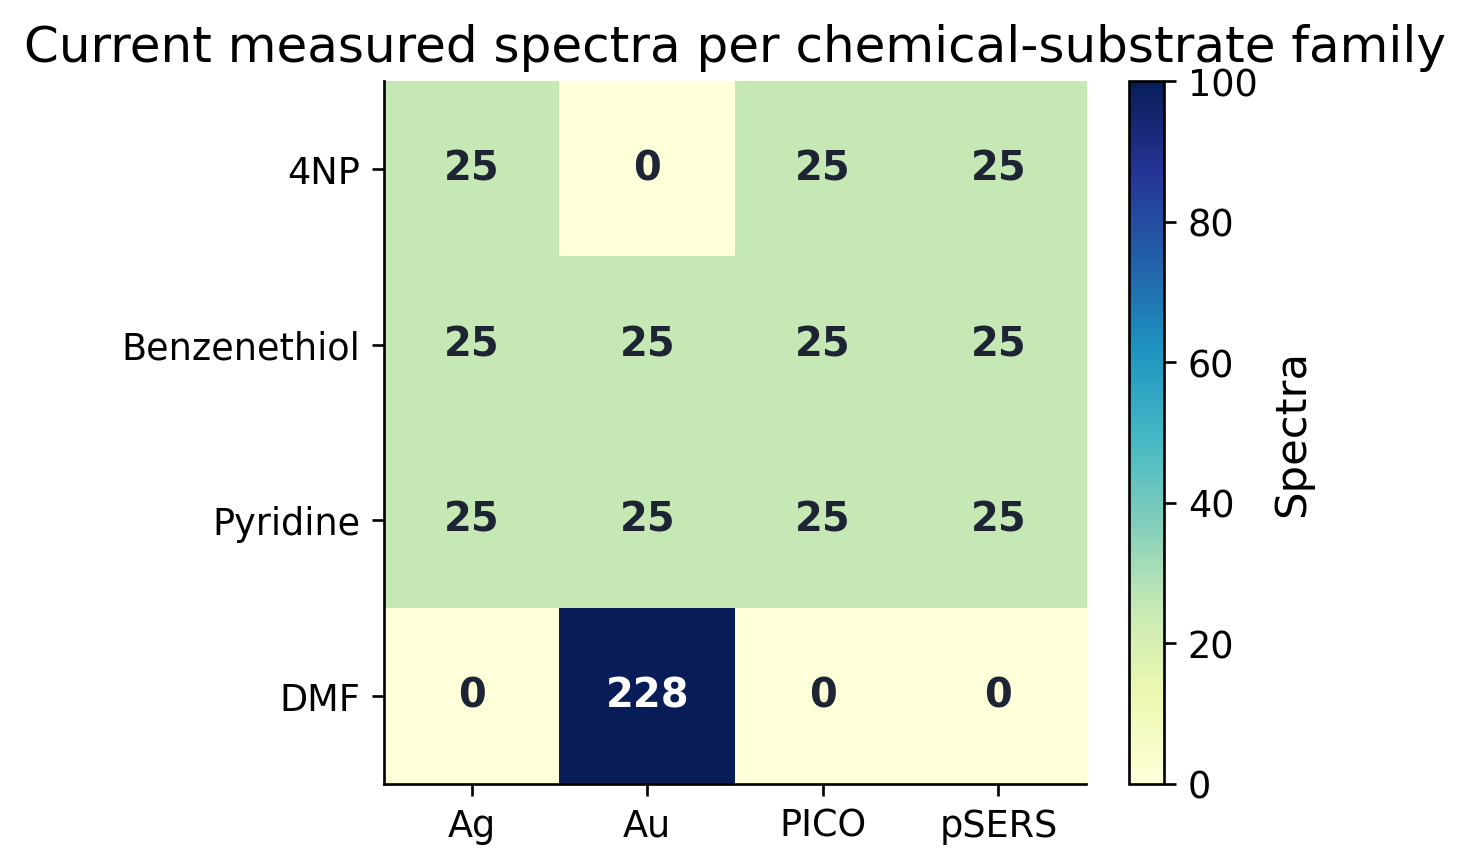
\includegraphics[width=0.24\linewidth]{figures/dataset_matrix_heatmap.png}
\end{center}
\figcaption{Measured spectra per chemical-substrate family. Cell values are spectra counts. The substrate-agnostic model uses 4NP, benzenethiol, and pyridine; DMF is excluded because it was measured only on Au and cannot support cross-substrate chemical learning.}

\subhead{Dataset implication}
The matrix is structurally incomplete, so broader chemical coverage across every substrate family is still needed.
}
\end{minipage}

\vspace{0.09in}

\begin{minipage}[t]{0.49\linewidth}
\contentpanel{9.65in}{%
\paneltitle{CHEMICAL-SUBSTRATE CLASSIFICATION}
\subhead{What the first model solved}
The first successful Siamese model predicted \textbf{pair labels}. Strong performance showed that the model could recognize measured chemical-surface signatures, but the substrate remained part of the class.

{\fontsize{24}{28}\selectfont\bfseries\color{templateaccent}98.76\%}\hspace{0.08in}{\bodytext top-1 pair-classification accuracy on 403 query spectra.}\par

\tabcaption{Stage 1 pair-classification model. The target is a pair identity, so high accuracy reflects recognition of combined analyte-surface signatures rather than substrate-independent chemistry.}
\begin{center}
\smalltext
\begin{tabular}{p{0.30\linewidth}p{0.60\linewidth}}
\toprule
\textbf{Item} & \textbf{Original pair model} \\
\midrule
Target & Chemical-substrate pair identity \\
Encoder & Shared Conv1D Siamese encoder, 64-D L2-normalized embedding \\
Loss & Contrastive loss, margin 1.0 \\
Inference & One known reference spectrum per pair class \\
Result & 98.76\% top-1 accuracy on 403 query spectra \\
\bottomrule
\end{tabular}
\end{center}

\begin{center}
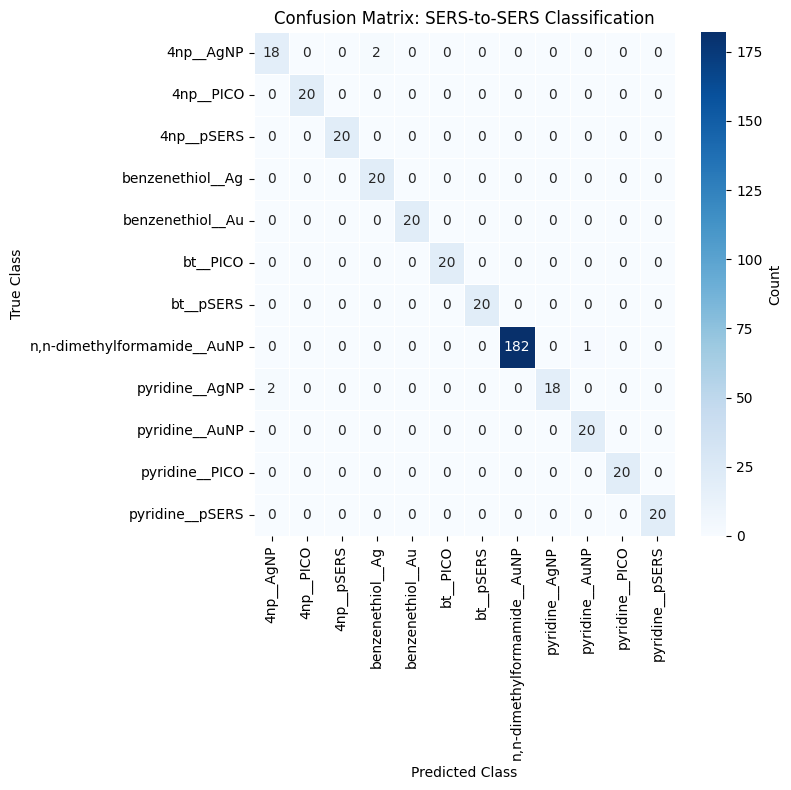
\includegraphics[width=0.28\linewidth]{figures/pair_classifier_confusion_matrix_notebook.png}
\end{center}
\figcaption{Original notebook confusion matrix for SERS-to-SERS chemical-substrate pair classification. The strong diagonal indicates most pair labels are recovered correctly, but every class still includes the substrate. This motivates the substrate-agnostic step: keep the Siamese metric-learning strategy but change the target to chemical identity.}
}
\end{minipage}
\hfill
\begin{minipage}[t]{0.49\linewidth}
\contentpanel{9.65in}{%
\paneltitle{SUBSTRATE-AGNOSTIC MODEL}
\subhead{Best chemical-label transfer}
{\fontsize{24}{28}\selectfont\bfseries\color{templateaccent}97.5\%}\hspace{0.08in}{\bodytext chemical-label accuracy under leave-one-substrate-family-out testing.}\par

\begin{minipage}[t]{0.52\linewidth}
\subhead{Current Siamese pipeline}
\tabcaption{Model input and training. The encoder receives a processed first-derivative spectrum, not the raw spectra shown in the schematic.}
\begin{center}
\smalltext
\begin{tabular}{p{0.32\linewidth}p{0.58\linewidth}}
\toprule
\textbf{Step} & \textbf{Role} \\
\midrule
Crop 330.906--1797.919 cm$^{-1}$ & Remove low-wavenumber device artifact region. \\
SNV normalization & Reduce intensity and offset variation. \\
Savitzky-Golay first derivative & Emphasize peak shape/position and suppress broad background. \\
Row L2 normalization & Put spectra on a comparable metric-learning scale. \\
Conv1D encoder & 1$\rightarrow$16 conv/pool; 16$\rightarrow$32 conv/pool; flatten; dense/ReLU to 64-D L2-normalized embedding. \\
Training & Triplet loss, margin 0.2; Adam $10^{-3}$; batch 32; 100 epochs; noise/shift augmentation; GPU/CUDA required. \\
\bottomrule
\end{tabular}
\end{center}
\end{minipage}
\hfill
\begin{minipage}[t]{0.44\linewidth}
\begin{center}
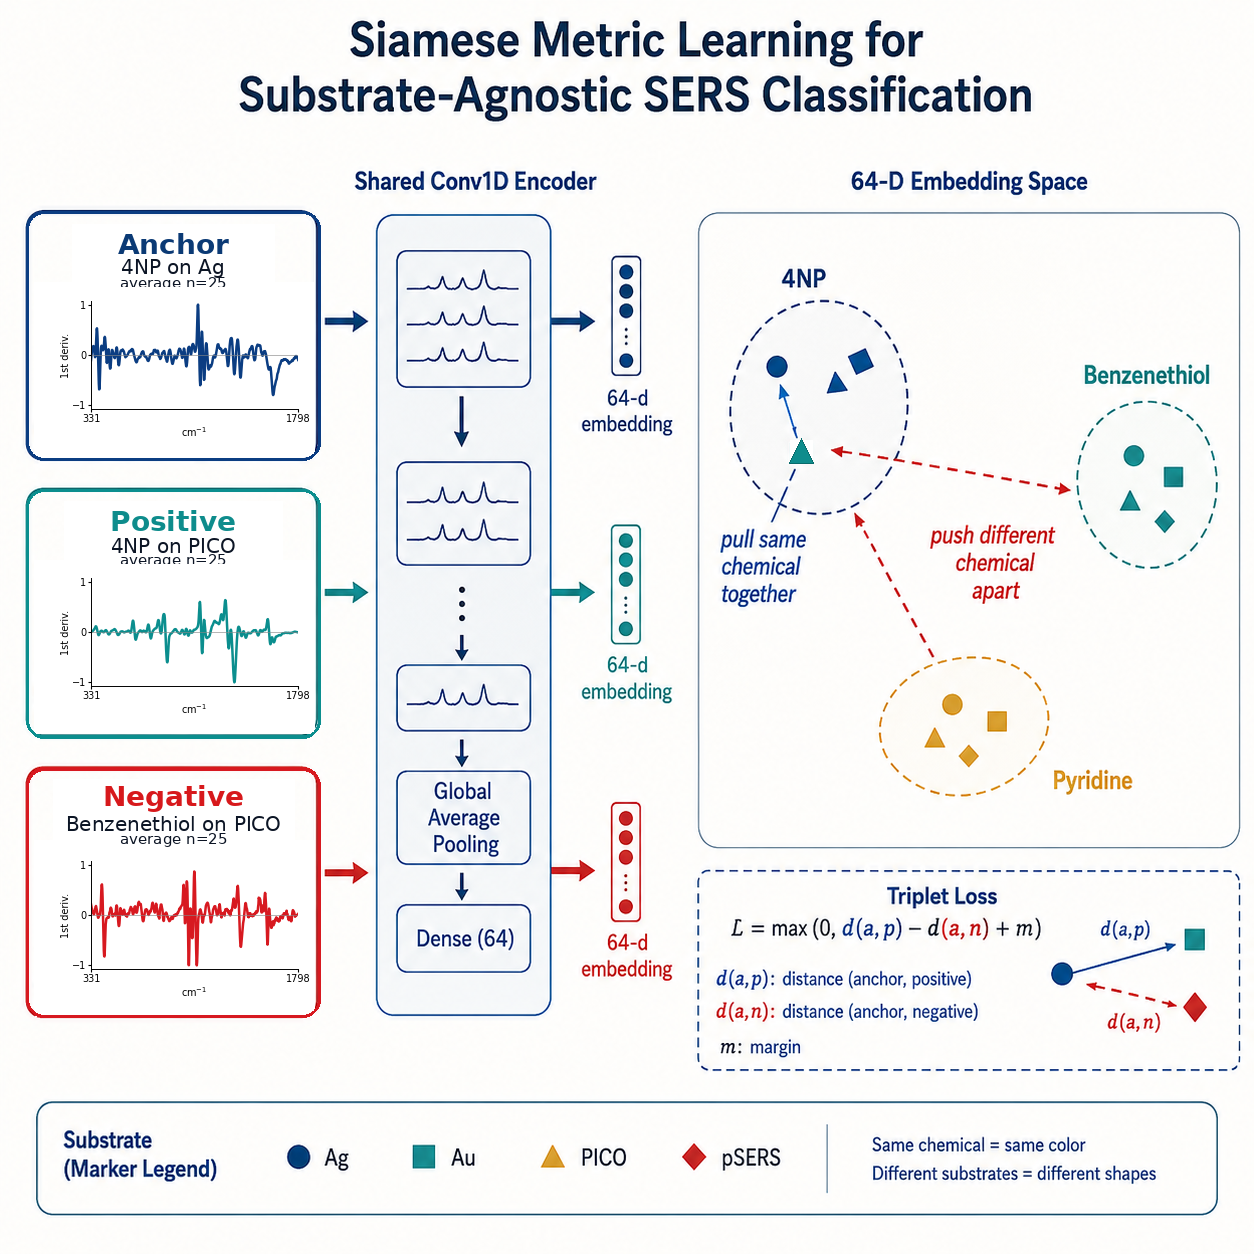
\includegraphics[width=0.34\linewidth]{figures/siamese_metric_learning_4np_pico_positive_average.png}
\end{center}
\figcaption{Triplet-learning schematic. Anchor and positive spectra share chemical identity and are pulled together; a different-chemical negative is pushed away. The plotted spectra are raw averages for interpretation; the encoder input is cropped, SNV-normalized, first-derivative, and L2-normalized.}
\end{minipage}

\vspace{0.02in}
\begin{minipage}[t]{0.34\linewidth}
\tabcaption{Leave-one-substrate-family-out performance. Scores use only chemicals present in the held-out substrate family.}
\begin{center}
\smalltext
\begin{tabular}{lrr}
\toprule
\textbf{Held out} & \textbf{Acc.} & \textbf{F1} \\
\midrule
Ag & 0.920 & 0.919 \\
Au & 0.980 & 0.990 \\
PICO & 1.000 & 1.000 \\
pSERS & 1.000 & 1.000 \\
\bottomrule
\end{tabular}
\end{center}
\end{minipage}
\hfill
\begin{minipage}[t]{0.62\linewidth}
\begin{center}
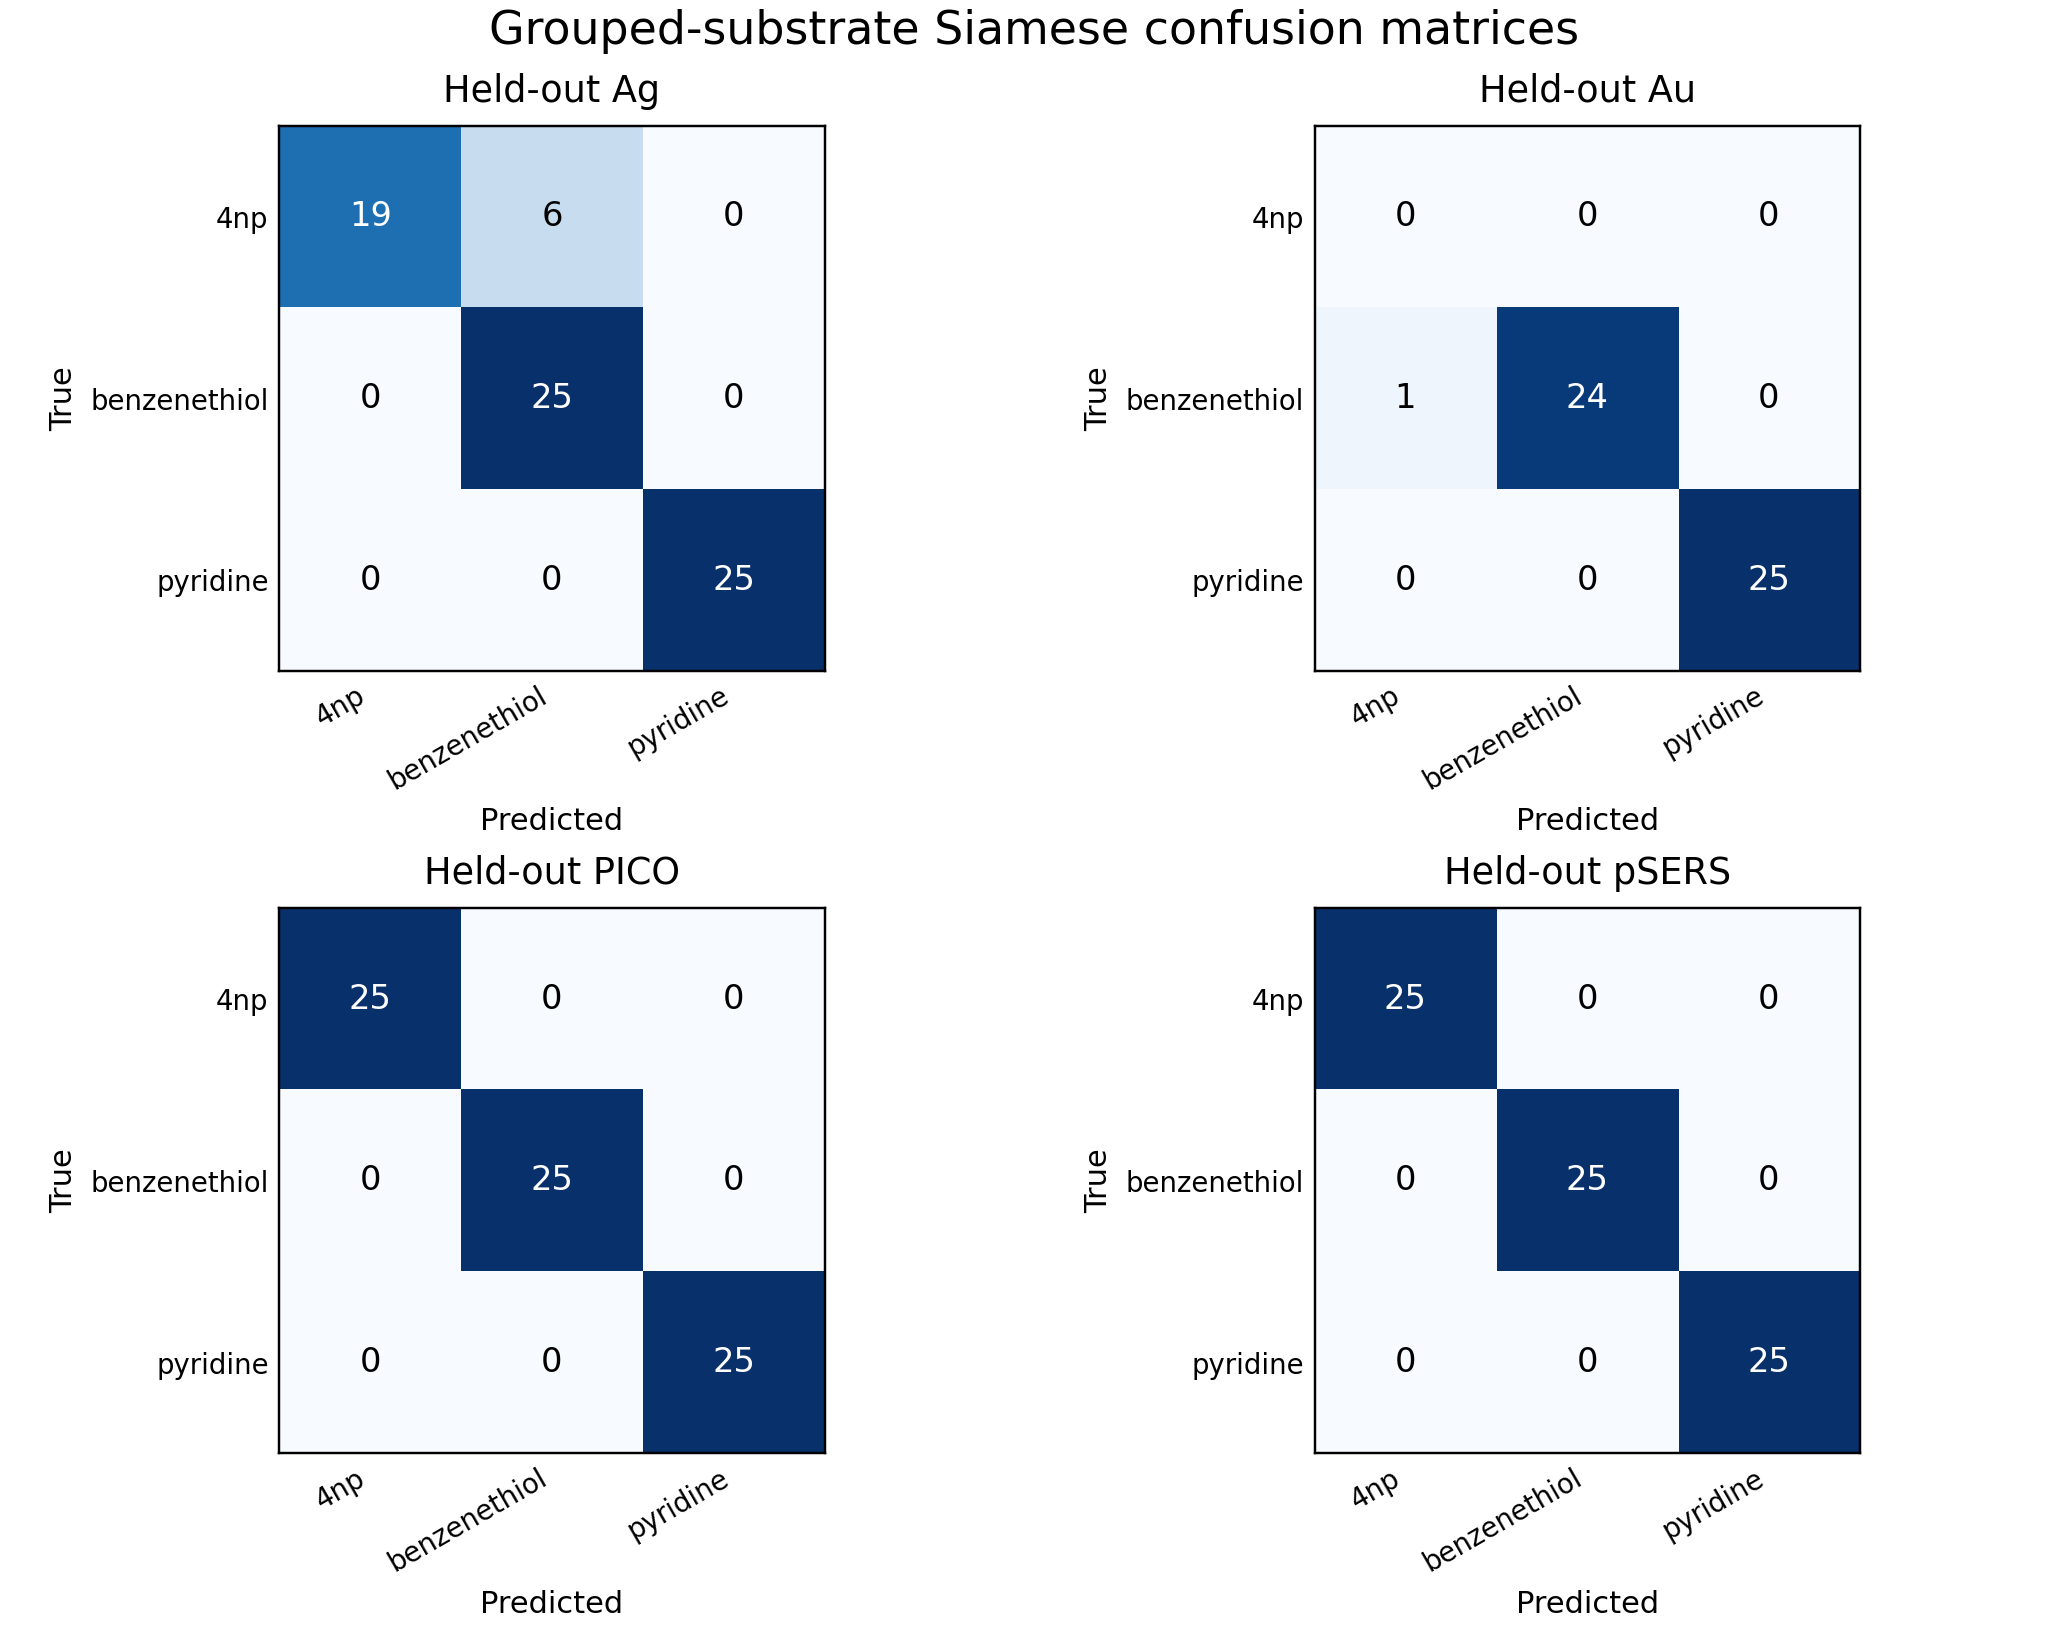
\includegraphics[width=0.27\linewidth]{../sers_substrate_agnostic_supervisor_report/figures/grouped_best_confusions.png}
\end{center}
\figcaption{Grouped-substrate Siamese confusion matrices. Transfer is clean for PICO and pSERS. The remaining weak point is the held-out Ag fold, where 6/25 4NP spectra are predicted as benzenethiol.}
\end{minipage}
}
\end{minipage}

\vspace{0.09in}

\contentpanel{14.80in}{%
\paneltitle{TAKEAWAYS AND FUTURE DIRECTIONS}
\begin{minipage}[t]{0.62\linewidth}
\begin{center}
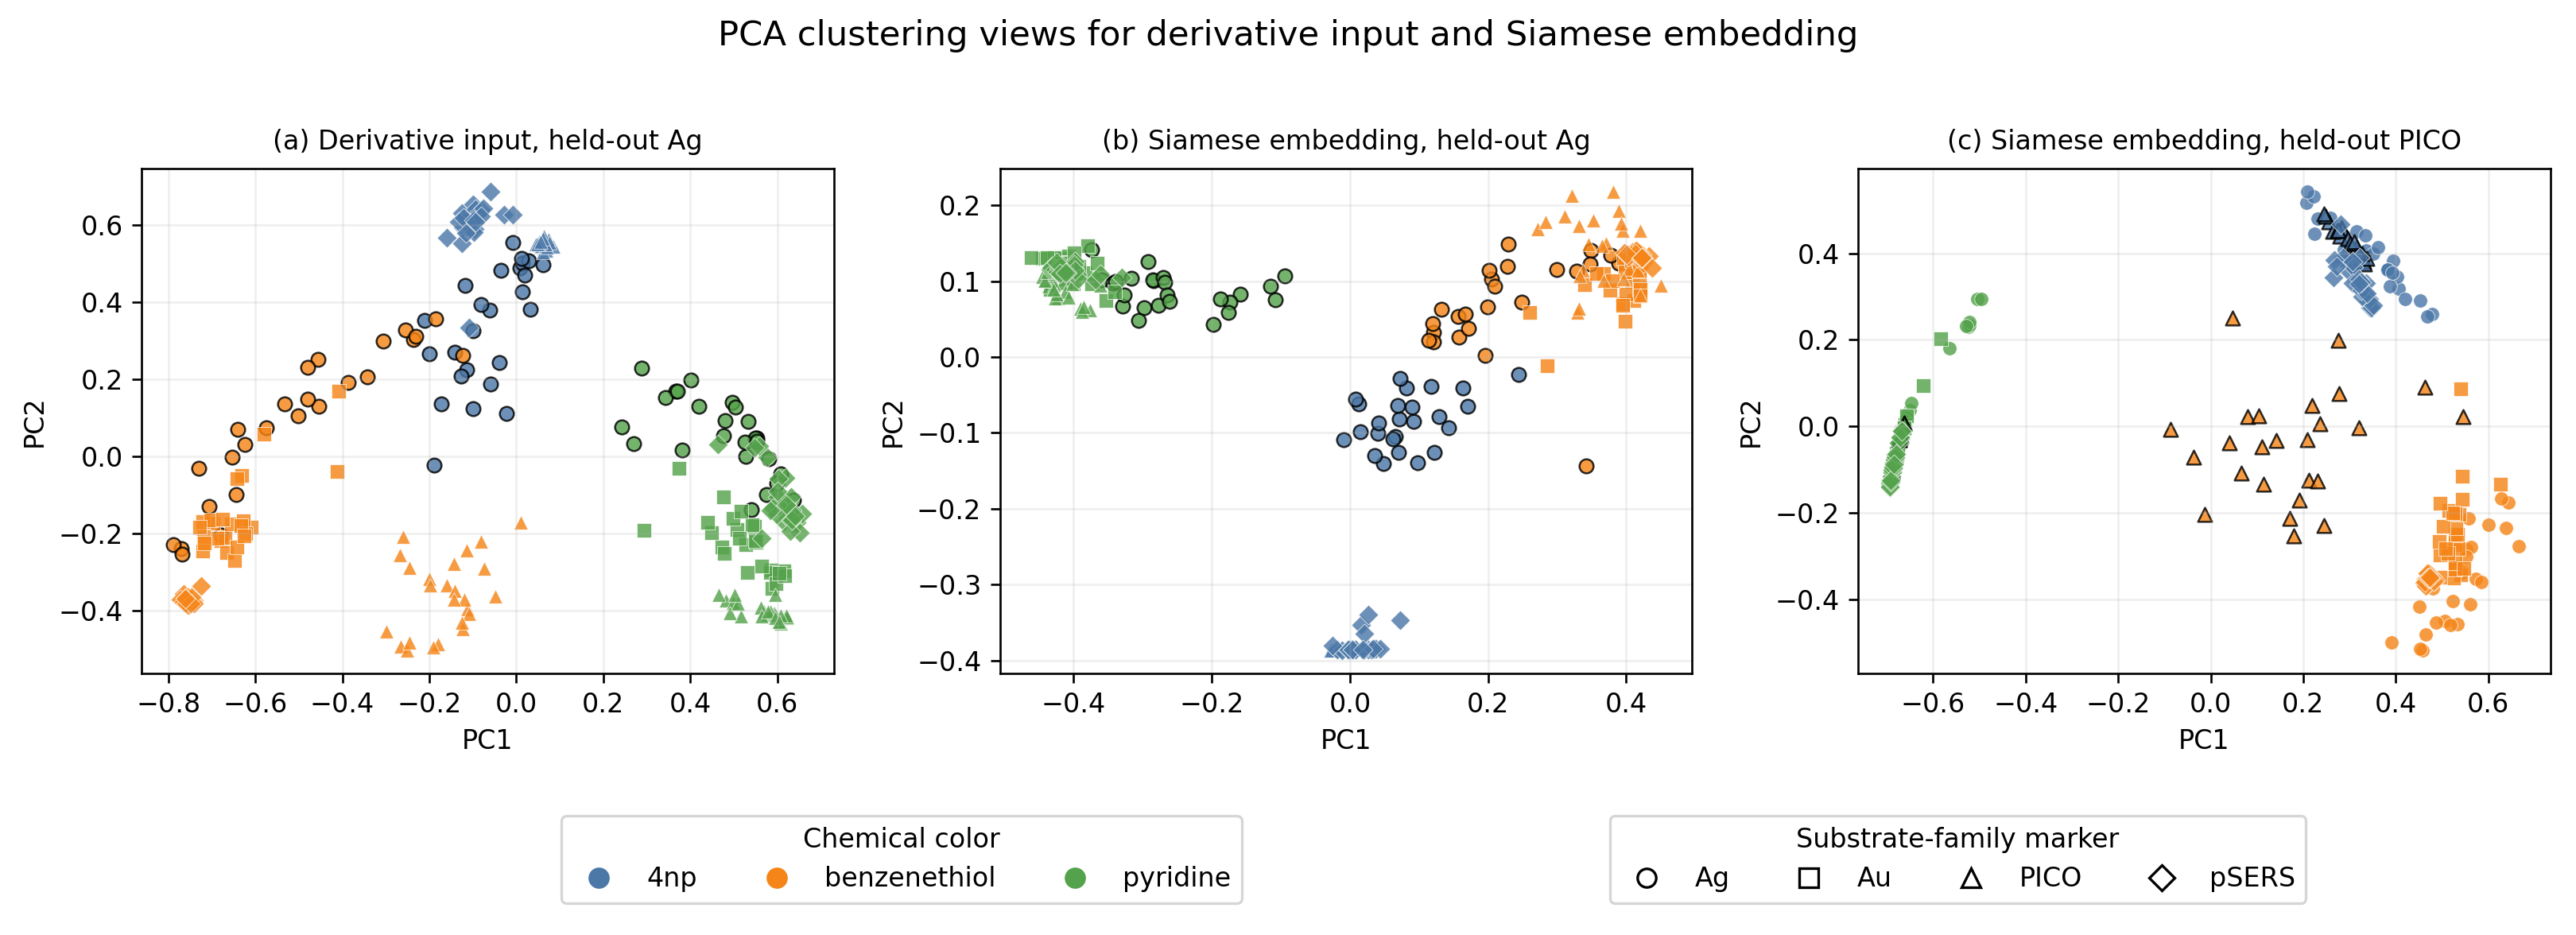
\includegraphics[width=0.91\linewidth]{../sers_substrate_agnostic_supervisor_report/figures/combined_pca_clustering.png}
\end{center}
\figcaption{PCA views comparing derivative-input space and Siamese-embedding space. Color indicates chemical identity and marker shape indicates substrate family. In derivative space, chemical and substrate effects are partially entangled. In embedding space, same-chemical spectra are tighter and more separable while substrate-family organization is reduced. The Ag/4NP weakness appears as a local overlap rather than a uniform collapse of chemical organization.}
\end{minipage}
\hfill
\begin{minipage}[t]{0.35\linewidth}
\smalltext
\subhead{Geometry shift}
{\fontsize{24}{28}\selectfont\bfseries\color{templateaccent}0.837}\hspace{0.06in}{\bodytext label-minus-substrate silhouette gain in embedding space.}\par

\tabcaption{Silhouette analysis of representation geometry. A higher chemical silhouette and lower substrate silhouette means the representation is organized more by chemical identity than by substrate family.}
\begin{center}
\begin{tabular}{lrrr}
\toprule
\textbf{Representation} & \textbf{Chem.} & \textbf{Substrate} & \textbf{Diff.} \\
\midrule
Derivative input & 0.304 & 0.101 & 0.203 \\
Siamese embedding & 0.797 & -0.040 & 0.837 \\
\bottomrule
\end{tabular}
\end{center}

\subhead{Takeaways}
\begin{itemize}
\item Stage 1 solved pair recognition, not substrate-agnostic detection.
\item Stage 2 keeps Siamese metric learning but changes the target to chemical identity and evaluates leave-one-substrate-family-out transfer.
\item The embedding generally pulls same-chemical spectra closer and reduces substrate-family structure, as shown by the silhouette shift.
\item The remaining weak point is specific: 4NP transfer to held-out Ag, not a uniform model collapse.
\end{itemize}

\subhead{Future directions}
\begin{itemize}
\item Fill the chemical-by-substrate matrix with more responsive chemicals measured across every substrate family.
\item Add independent preparations, measurement days, and map locations rather than only repeated spectra from one preparation.
\item Prioritize Ag-family 4NP/benzenethiol measurements to separate chemical overlap from substrate-specific enhancement.
\item Validate on a truly new substrate or acquisition day after the matrix is expanded.
\end{itemize}

\vspace{0.01in}
\begin{minipage}[t]{0.64\linewidth}
{\fontsize{15}{18}\selectfont\bfseries\color{templateblue}ACKNOWLEDGMENTS}\par
{\captionfont National Research Council Canada, Metrology Research Centre.}
\end{minipage}
\hfill
\begin{minipage}[t]{0.30\linewidth}

\includegraphics[width=0.70\linewidth]{figures/logos/nrc_logo.png}
\end{minipage}
\end{minipage}
}

\end{document}
